\documentclass[10pt,a4paper]{report}
\usepackage[utf8]{inputenc}
\usepackage[russian]{babel}
\usepackage[OT1]{fontenc}
\usepackage{amsmath}
\usepackage{amsfonts}
\usepackage{amssymb}
\usepackage{graphicx}
\author{Никитина Анна и Замотаева Юлия}
\title{Отчет по лабораторной работе по дисциплине: "Сети и системы передачи данных"\newline
тема: "Спектры простых сигналов"}
\date{10.04.14}
\begin{document}
\maketitle
\pagebreak
\chapter{Задачи работы}
\section{Цель работы}
Получить представление о тестовых сигналах во временной и частотной областях. Реализовать операцию свертки сигналов.
\section{Алгоритм работы}
\begin{itemize}
\item Построение полигармонического сигнала
\item Построение прямоугольного импульсного сигнала
\item Построение треугольного импульсного сигнала
\item Получение спектров этих сигналов
\end{itemize}
\chapter{Код MATLAB}
\section{Код MATLAB для полигормонического сигнала}
x = 0:0.01:4*pi;\newline
f=100*(0:255)/512; \newline
figure\newline
y1 = sin(2*pi*x)+sin(2*pi*3*x);\newline
plot(x(1:200),y1(1:200))\newline
grid\newline
figure\newline
s1 = fft(y1,512);\newline
ss1 = s1.*conj(s1)/512;\newline
plot(f,ss1(1:256))\newline
grid \newline
figure\newline
y2 = sin(2*pi*x)+cos(2*pi*x);  \newline
plot(x(1:200),y2(1:200))  \newline 
grid \newline
figure\newline
s2 = fft(y2,512);\newline
ss2 = s2.*conj(s2)/512;\newline
plot(f,ss2(1:256))\newline
grid \newline
\section{Код MATLAB для прямоугольного импульсного сигнала}
t=-0.04:1/1000:0.04;\newline
y4=-5*rectpuls(t,0.04);\newline
plot(t,y4);\newline
figure;\newline
spectrum = abs(fft(y4,1024))/1024;\newline
plot(spectrum);\newline
\section{Код MATLAB для треугольного импульсного сигнала}
t=-0.04:1/1000:0.04;\newline
y4=-5*rectpuls(t,0.02);\newline
y5=-10*rectpuls(t,0.03);\newline
y6= conv(y4,y5);\newline
plot(y6);\newline
figure;\newline
spectrum = abs(fft(y6,1024))/1024;\newline
plot(spectrum);\newline
\chapter{Полученные графики}
\begin{figure}
\begin{center}
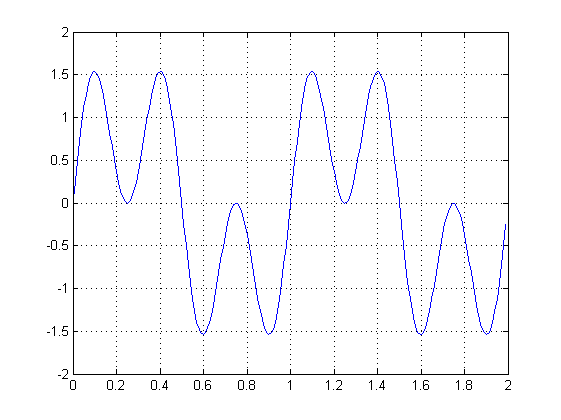
\includegraphics[angle=0, scale = 0.9]{1.png}\newline
рис. 1. полигармонический сигнал sin(x)+sin(3x)\newline
\end{center}
\end{figure}
\begin{figure}
\begin{center}
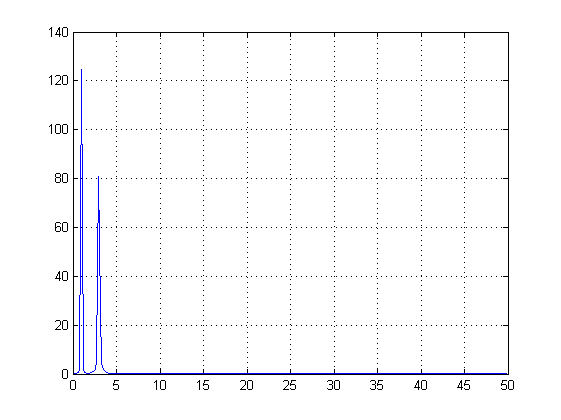
\includegraphics[angle=0, scale = 0.9]{2.png}\newline
рис. 2.спектр данного полигармонического сигнала\newline
\end{center}
\end{figure}
\begin{figure}
\begin{center}
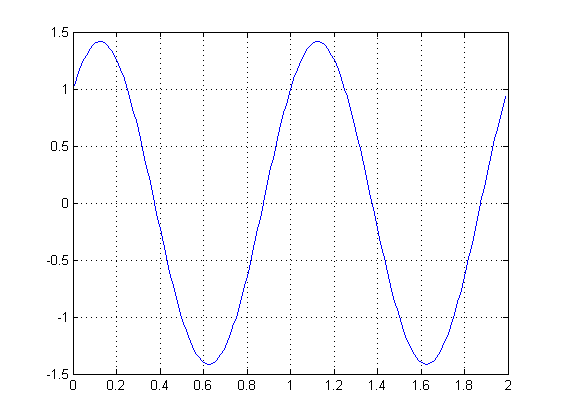
\includegraphics[angle=0, scale = 0.9]{12.png}\newline
рис. 3. полигармонический сигнал sin(x)+cos(x)\newline
\end{center}
\end{figure}
\begin{figure}
\begin{center}
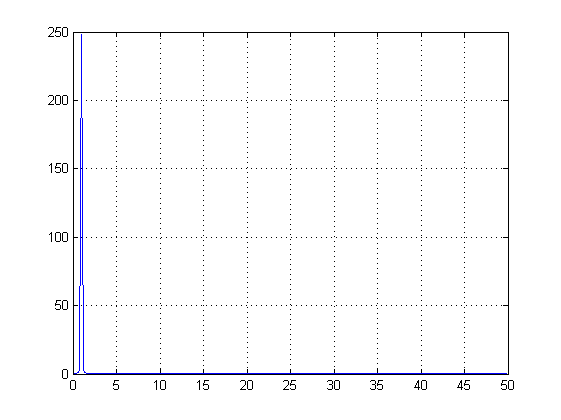
\includegraphics[angle=0, scale = 0.9]{11.png}\newline
рис. 4.спектр данного полигармонического сигнала\newline
\end{center}
\end{figure}
\begin{figure}
\begin{center}
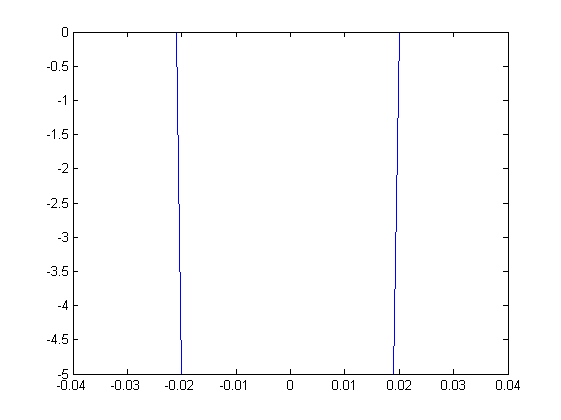
\includegraphics[angle=0, scale = 0.9]{3.png}\newline
рис.5.прямоугольный сигнал\newline
\end{center}
\end{figure}
\begin{figure}
\begin{center}
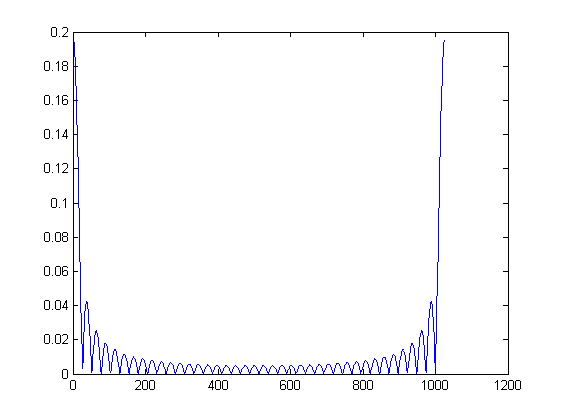
\includegraphics[angle=0, scale = 0.9]{4.png}\newline
рис. 6 спектр прямоугольного сигнала\newline
\end{center}
\end{figure}
\begin{figure}
\begin{center}
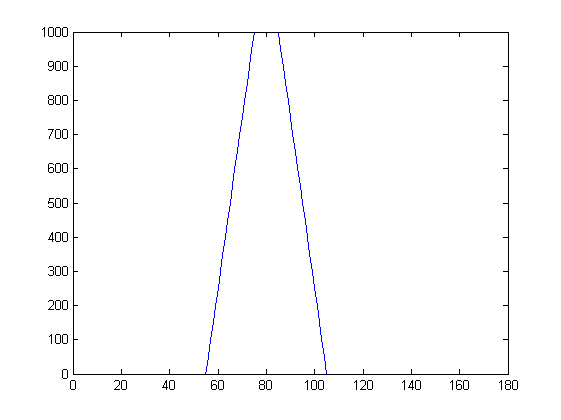
\includegraphics[angle=0, scale = 0.9]{5.png}\newline
рис. 7  треугольный сигнал\newline
\end{center}
\end{figure}
\begin{figure}
\begin{center}
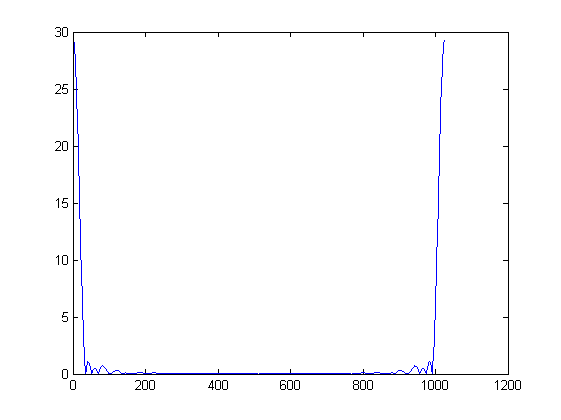
\includegraphics[angle=0, scale = 1.1]{6.png}\newline
рис. 8 спектр треугольного сигнала \newline
\end{center}
\end{figure}
\chapter{Вывод}
\section{Теоритическая часть}
В лабораторной работе было проведено моделирование полигармонического, прямоугольного и треугольного сигналаов. После чего получены их спектры. Для получения сигналов использовались математические формулы данных функций. Треугольный сигнал был получен путем применения операции свертки для двух прямоугольных сигналов. Данная операция осуществляется с помощью специальной функции Matlab.\newline
Обоснованием получения треугольного сигнала из свертки двух прямоугольных служит тот факт, что интеграл от произведения двух констант есть линейная функция. График такого преобразования будет представлять две линеные функции, одна из которых имеет положительный коэффициент наклона, а другая отрицательный.
\section{Формулы}
Ниже приведены формулы для вычисления спектров исходных импульсов. Так как треугольный импульс можно представить в виде свертки двух прямоугольных, спектр треугольного испульса выражается через квадрат спектра прямоугольного импульса. 
\begin{displaymath}
S(t)=\sum \limits_{k=0}^{K}(a_{k}*cos(2*pi*k*f*t)+b_{k}*sin(2*pi*k*f*t))\newline
\end{displaymath}
\begin{center}
Спектр полигармонического импульса
\newline
\end{center}
\begin{figure}
\begin{center}
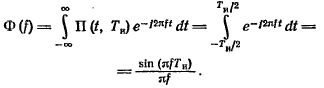
\includegraphics[angle=0, scale = 1.0]{8.png}\newline
рис. 9    Спектр прямоугольного импульса\newline
\end{center}
\end{figure}
\begin{figure}
\begin{center}
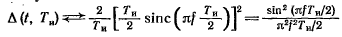
\includegraphics[angle=0, scale = 1.0]{9.png}\newline
рис. 10  Спектр треугольного импульса
\end{center}
\end{figure}
\end{document}
